\chapter{Introduction}
\label{intro}

Human brains are built to come to single conclusions about things that have more than one interpretation.  That single conclusion is developed based upon one's experiences, cutural immersion, and language familiarity \cite{smith_music_2003}. When attempting to write English phrases that will be read aloud and heard by people with different linguistic biases, it is important to make prose as deterministically understandable as possible. The first step towards this is understanding and identifying how many ways a particular textual phrase can be misheard, and why.


\section{You and me...and Leslie?}
\label{sect:youAndMeAndLeslie}

In the song \textit{``Groovin' (on a Sunday Afternoon)''}, by the Young Rascals, there is a part in the bridge that many people hear as \textit{``Life would be ecstasy, you an' me an' Leslie''}. In fact, the line is \textit{``Life would be ecstasy, you and me endlessly''}. The confusion lies with the last three syllables of the phrase. The pronunciation of each version, if spoken normally, is as follows:



%\begin{table}
\begin{center}
    \begin{tabular}{|l|c|c|}
        \hline
        \textbf{Orthographic:} & and       Les-   lie & end-       less-       ly \\ 
        \hline
        \textbf{SAMPA:}      & \texttt{@nd   ``lEs     li}   & \texttt{``End      l@s       li}   \\
        \hline
    \end{tabular}
\label{table:groovinAlphaSAMPA}
\end{center}
%\end{table}


In the song, the singer is doing what many singers are taught to do: to make it easier to sustain the singing of words that end with difficult-to-sing consonants, the unsingable consonant is displaced onto the front of the next word. In this case, the consonant ``d'' is not singable, so the singer displaces it onto the next syllable: ``and ME'' becomes ``an dME'', and ``end LESS'' becomes ``en dLESS''. 

In this way, singers are often apt to ignore syllable boundries. In this case, the singer now effectively thinks of the sung phrase as:

\begin{center}
YOU an dME en dLESS lee
\end{center}

This elimination of syllable boundaries in the singer's mind does not cause confusion for listeners, because they are used to hearing this technique used. This does mean, however, that lyric placement does not provide an accurate barometer to a listener of where a word actually ends.

In addition, the singer is fudging their vowels, like singers are taught to do. As a result, ``and'' and ``end'' sound almost indistinguishable. So, really, what listeners are hearing is this:

\begin{center}
YOU en dME en dLESS lee
\end{center}

 Now, the listener's brain has to take this phonetic sequence, and parse it into something useful. They've currently got this phonetic sequence to interpret (represented in SAMPA syllables):

\begin{center}
{\large \textit{\textbf{ju }}}{\large \textit{En }}{\large \textit{\textbf{dmi 
}}}{\large \textit{En }}{\large \textit{\textbf{dl@s }}}{\large \textit{li}}
\end{center}

 They parse the first part just correctly, because the emphases match:

\begin{center}
{\large \textbf{you }}{\large and }{\large \textbf{me }}{\large \textit{En }}{\large \textit{\textbf{dl@s 
}}}{\large \textit{li}}
\end{center}

But no one says endLESSly. People say ENDlessly. So, the listeners don't recognize it. They have to work with what they have. They already turned one ``En d'' into an ``and'', so they do it again:

\begin{center}
{\large \textbf{you }}{\large and }{\large \textbf{me }}{\large and }{\large \textit{\textbf{l@s 
}}}{\large \textit{li}}
\end{center}

Now, they're just left with LESS lee. And that fits Leslie, a proper noun that fits in context and in emphasis placement. So, the final heard lyric is:

\begin{center}
{\large \textbf{you }}{\large and }{\large \textbf{me }}{\large and }{\large \textbf{Les- 
}}{\large lie}
\end{center}

The misunderstanding can be traced back to improper analysis of the lyric's multiple aural interpretations. The songwriter probably didn't even think of that, and now he's stuck: a one-hit-wonder with a misunderstood song. We bet that in interview after interview, someone asks him who Leslie is. It's probably very frustrating --- especially since he could have just moved the word an eight note later, and it would have been understood perfectly.

That's the sort of situation this program is going to help avoid.



\section{ Why it breaks down }
\label{sect:whyItBreaksDown}

There are two points at which an author's intendeded phrasing can be muddled: First, when the author's orthographic text becomes an orator's spoken (phonetic) interpretation, and second, when the orator's phonetic interpretation is translated phonetically by an audience into a perceived orthographic phrase. Both of these interpretations must be made succesfully in order for the author's intended meaning to be conveyed.

The phrase ``iced ink" undisputedly succeeds in the first translation from orthographic phrase to phonetic interpretation, since there is only one possible pronunciation. However, it fails on the second.  Iced ink can only be pronouced one way, but it can be heard multiple ways--the most notable of which is ``I stink", not ``iced ink".

The phrase ``a nice cold hour" can fail on both parts.  First, the orator could have accidentally-capitalized the word Nice in their head, and made it sound like Nice, the city in France.  An audience would likely hear this as ``niece", and would be confused, at best.  Even if the orator pronounces the phrase as the author intended, the audience could hear multiple orthographic phrases in the same phonetic sequence: ``a nice cold hour", ``an ice cold hour", or even ``a nigh scold our".

A third, more rare and nefarious type of audience misunderstanding can be caused by parse-tree misdirection, where an audience member is absolutely sure they are hearing one phrase, only to get lost halfway through the phrase because they were interpreting a phonetic sequence in a way that resulted in an orthographic dead end. This happens due to the relative frequency of the possible words heard in the aurally-interpreted lyrics.

For example, when asked to sing along with the Adele song, Rolling in the Deep, people who were starting to sing enthusiastically dropped out around the line ``reaching a fever pitch"\cite{frontPorchBandAdeleCover}.  Let us consider the phrase ``fever pitch".  This phrase has no exact oronyms, but it does have a potential dead end-- a listener could hear the first syllable of the phrase as the word ``fee", which has a frequency of 7265.  That's more than double the frequency of the word ``fever", which is 3095.  

Looking at the oronym parse tree for the phrase ``fever pitch" in figure ~\ref{fig:feverPitchOronymTree}, we can see that the branch for ``fever" ends in a much smaller radius than the branch on the left for the word ``fee".  As you can see by the relative size of the end spheres of the branches, the word ``fee" even outweighs the last word in the other branch as well (which is ``pitch" with a frequency of 5104). Since the human brain is pre-disposed to parse more-familiar words, having that heavily-weighted dead-end branch is likely the cause of the casual listener not being able to effortlessly memorize the lyrics.
\begin{wrapfigure}{r}{0.5\textwidth}[h]
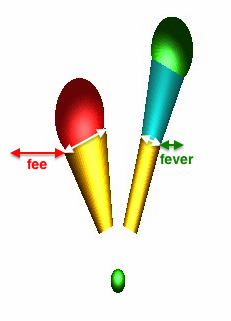
\includegraphics[width=.5\textwidth]{feverPitchTreeAnnotated.jpg}
\captionfonts
\caption[Annotated Oronym Parse tree  generated for the phrase ``fever pitch"]{ Annotated Oronym Parse tree generated for the phrase ``fever pitch" }
\label{fig:feverPitchOronymTree}
\end{wrapfigure}



